\documentclass[a4paper,12pt]{article}

\usepackage{url}
\usepackage{epsfig}
\usepackage{graphics}
\usepackage{fancyhdr}
\usepackage{amsmath}

\graphicspath{{pictures/}}

\title{Detecting context-dependent word defects in written English by native Swedes with n-grams}
\author{\hspace*{-0.5cm}\begin{tabular}{cccc}
Frej Connolly & Maja Gidlund & Sandra Liljeqvist & Sara Norrby \\
connolly@kth.se & majagi@kth.se & sanlil@kth.se & saranorr@kth.se \\
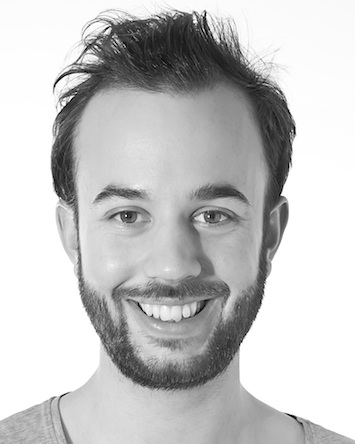
\includegraphics[width=0.13\linewidth]{frej} & 
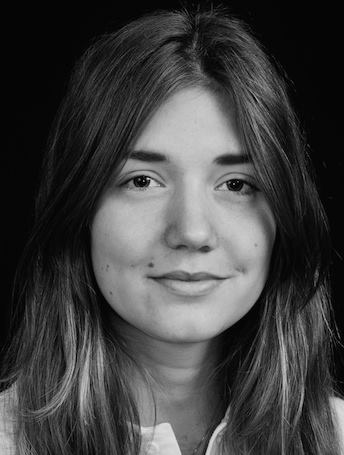
\includegraphics[width=0.13\linewidth]{maja} & 
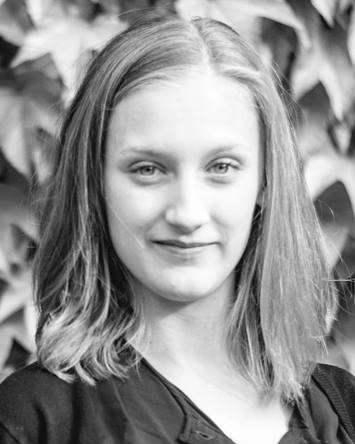
\includegraphics[width=0.13\linewidth]{sandra} & 
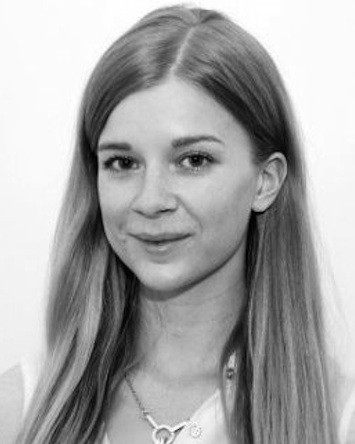
\includegraphics[width=0.13\linewidth]{sara}
\end{tabular}}
\date{2014-10-05}

\pagestyle{fancy}
\setlength{\headheight}{15pt}
\fancyhf{}
\lhead{DD2380 ai14} % DO NOT REMOVE!!!!
\rhead{F. Connolly, M. Gidlund, S. Liljeqvist, S. Norrby}

\begin{document}

\maketitle
\thispagestyle{fancy}

\begin{abstract}
TODO
\end{abstract}



\clearpage

%%%%%%%%%%%%%%%%%%%%%%%%%%%%%%%%%%%%%%%%%%%%%%%%%%%%%%%%%%%%%
%%%%%%%%%%%%%%%%%%%%%%%%%%%%%%%%%%%%%%%%%%%%%%%%%%%%%%%%%%%%%
\section{Introduction}
\label{sec:introduction}
The need to be able to write accurate English is growing as the market is becoming more global. For native Swedish speakers it can be easy to write a word that does not make sense in a certain context, by mistake. A traditional spell checker will not detect this kind of mistake since the words themselves often are correct, but placed in the wrong context.

For example if a Swede wants to ask a friend if he has a dinner jacket, the person might say \emph{Do you have a smoking?} believing that the word smoking (Swedish word for dinner jacket) has the same meaning in English. The native English speaker could interpret that what the Swede really intended to say was \emph{Do you have a cigarette?}  

A normal spell checker would not be able to find an error like this, but an algorithm that looks at the probability of the word order might. The standard way to implement this type of word prediction is by using the so called n-gram model. The n-gram model is based on 
statistical language modeling and uses the $n-1$ previous words in a sentence to predict the next word. Examples of n-grams is unigram $n=1$, bigrams $n=2$ and trigrams $n=3$. This is covered in more detail later on in the report \cite{gallagher2004natural}.

We anticipate that a tool that could locate this kind of mistake could be of great help. As far as we know there is no tool like this specialized in Swedes writing in English. The tool should work as a context-dependent word detection.

\subsection{Objective}
\label{sec:objective}
The aim for this project is to investigate if it is possible to implement a system that will find words that are out of context by using n-grams. We will implement a program and analyze if it can identify this kind of words in different sentences. The application area for this system will be for people with Swedish as a first language and English as a foreign language, who wants to write in English without making unnecessary mistakes.

\subsection{Hypothesis}
Our hypothesis is that it is enough to use bigrams and trigrams and a probability threshold to detect words that are out of context in a given text. However, the results will be affected by the quality of the corpus (covered in section 2.1) and we believe that a large and well chosen corpus is vital for the result of this study.

We believe that a combination of bigrams and trigrams will make a good balance in the algorithm and that it will suffice to reach the goal (covered in 4). The reason for that is partly that the two methods would complement each other well with different but necessary information. As the investigation focuses on the context, the use of unigrams would not be relevant, since it is only based on the current word. On the other hand, having the same four (or more) words in a row is very rare, therefore we decided to not use n-grams that are bigger than three, as the amount of data would not be enough to make informed decisions.

\subsection{Contribution}
\label{sec:contribution}
The purpose of our program is to reduce the number of incorrect uses of  words in writing. False friends and pseudo-anglicism are strongly related to the problem of expressing ourselves improperly in a language other than our mother tongue. In these cases a spell checker would not react since the words are correctly spelled, but used in the wrong context. Since millions of people speak English as a foreign language and many of the languages, that these people has as their first language, have false friends with English. This could help these people to better understand and to learn the English language. 

Previous work has been done in this field for several different languages, but in our work we will focus on the Swedish languages and the difficulties people with Swedish as their first language have with English.

\subsection{Outline}
\label{sec:outline}
TODO

\section{Language Modeling}
\subsection{N-gram modeling}
In general a statistical language modeling is based on n-gram language modeling which tries to predict the next word in a sentence based on the $n-1$previous words in the sentence \cite{gallagher2004natural}.  When choosing two words to compute the probability that a given word is the next word is called bigram. If we for example have the sentence \emph{I painted the house in the color} and uses bigram to guess the next word in the sentence we would compute $\Pr(predictive word \mid color)$. Although it makes more sense to assume, by using the whole sentence, that it would be easier for a human to guess the next word. This because the guess then could also be based on the context of the sentence. However, the bigram does not take as much computer power unlike if one wants to compute the whole sentence. It also takes less time to compute a bigram in comparison to compute a whole sentence \cite{gallagher2004natural}.

The information that is needed to compute an n-gram is how often a word occurs in general and how often a word occurs with others specific words. The n-gram model is using the Markov assumption, which is the assumption that the future behavior of a dynamical system only depends on its recent history \cite{mooneynatural}. In this case the history of the $n-1$ previous words. 

The n-gram model is often used together with one or several corpora. This is a large collection of text, written by humans, for different purposes that can be used for analyzing natural language. A great volume of text like this is necessary to make a probabilistic model, like n-grams, effective, since this approach requires that the system is learning from a big amount of data \cite{russell2010ai}.

\subsection{Problem with sparse data}
The process of smoothing is used to improve the reliability of the n-gram frequency, which occurs because of the low frequency many n-grams tend to have. What smoothing does is that it is reducing the numbers of zeros of probabilities. This means that if a system uses trigram, the weighted probability is the sum of the trigram, the bigram and the unigram. Therefore, if a system wants to combine different methods to predict the next word it could still be predicted right even though its probability of the trigram tends to be extremely low \cite{smoothing}.

\subsection{False Friends or Cognates}
In the paper Automatic Identification of Cognates and False Friends in French and English the authors Diana Inkpen, Oana Frunza and Grzegorz Kondrak bring up false friends and cognates \cite{frunzaInkpen2009identification}. In most languages there are words that are similar, in spelling, to words in other languages. Sometimes this is helpful, cognates are pairs of words in two different languages that have similar spelling and also the same meaning. One example of a pair, mentioned by Inkpen, Frunza and Kondrak, is the French nature and the English nature. They are spelled exactly the same and have the same meaning.

But sometimes the use of words that are similar is a bad idea. False friends are pairs of words that look alike, but mean completely different things. One example of this is french main, which means hand, and main in English. There are also some words that in some contexts have the same meaning but in others have a completely different one \cite{frunzaInkpen2009identification}.

\subsection{Pseudo-anglicisms}
Pseudo-anglicisms are words, that a language has borrowed from the English language, that do not make sense in English. These kinds of words are related to false friends but is not entirely the same. One example in German is body-bag which is a kind of backpack with only one strap. Another example is the Swedish word backslick, which in English really is called slick-back hairdo. Sometimes the words do not mean anything at all in English but sometimes the words have a completely different meaning \cite{pseudoanglicism}.

%%%%%%%%%%%%%%%%%%%%%%%%%%%%%%%%%%%%%%%%%%%%%%%%%%%%%%%%%%%%%
%%%%%%%%%%%%%%%%%%%%%%%%%%%%%%%%%%%%%%%%%%%%%%%%%%%%%%%%%%%%%
\section{Related work}
\label{sec:relatedwork}
The paper Techniques for automatically correcting words in text by Karen Kukich brings up three different types of error detection and correction. The type most interesting to us was context dependent word-correction. Kukich discusses previous work and different approaches for the context dependent word-correction \cite{Kukich1992Tecniques}. However, in this report the focus is not on word-correction but on word-detection.

Several research papers have discussed how to capture the context of a sentence without having to analyze the whole sentence. In the article A Swedish Grammar for Word Prediction, written by Ebba Gustavii and Eva Pettersson, grammar rules was implemented by using the FASTY language modeling to predict the next word with the use of the n-gram modeling \cite{gustavii2003a}. The article's aim was to cover contexts where statistical models gives irrelevant suggestions. The hypothesis of the article was that the FASTY would achieve a good and intelligent choice of words. The particularly useful part of this article was the method for measuring and evaluating the results.

%%%%%%%%%%%%%%%%%%%%%%%%%%%%%%%%%%%%%%%%%%%%%%%%%%%%%%%%%%%%%
%%%%%%%%%%%%%%%%%%%%%%%%%%%%%%%%%%%%%%%%%%%%%%%%%%%%%%%%%%%%%
\section{Method}
\label{sec:method}
The project is divided into two parts: implementation and analyzing. 
The implementation is based on the previously mentioned n-gram model where the probability of a word being correct is based on the probability of it being followed by the n-1 previous words. Based on the hypothesis, a combination of bigrams and trigrams is used to be able to find possibly incorrect words. The text processing library Natural Language Toolkit (NLTK) in Python is conveniently used to save time for already solved problems \cite{loper2002nltk}. 

As input, the program takes a text or sentence and as output it returns the words that is probable to be incorrect. The decision if a word should be output or not is made by a threshold of the probability of the n-grams ending with this word. The threshold is tuned during the work to find the best possible result. 

For the analysis and evaluation of the algorithm, we used a quantitative method, were we composed $x$ sentences containing incorrect words or expressions. For the creation of these sentences we used a database with common errors, that Swedes usually makes when writing in English, combined with example sentences from a Swedish textbook in the English language. As a complement to this, English texts without errors were also used.

For measuring the results we calculated the quota between the correctly detected defects and all defects together with incorrectly detected defects. This equation is called the Hit Rate \cite{wikipedia2014hitrate, ghayoomi2005word}.

$$z = \frac{\sum correct}{\sum correct + \sum not\_detected + \sum incorrect}$$
\begin{description}
  \item[correct] \hfill \\
  		correctly detected defects
  \item[not\_detected] \hfill \\
  		defects not detected
  \item[incorrect] \hfill \\
   		incorrect defects detected
\end{description}

If z equals one, the algorithm correctly found all defects with no incorrect matches and if z is zero, it did not found any of the defects.

The different approaches described earlier is considered useful if $z \geq 0.70$ for all measurements. If $z \geq 0.90$ the result is successful and on par with similar research \cite{frunza2006automatic, frunzaInkpen2009identification}. Tuning each algorithm is done by running it multiple times, adjusting the threshold each time until the goal of z is reached.


\subsection{Implementation}
\label{sec:implementation}
TODO

%%%%%%%%%%%%%%%%%%%%%%%%%%%%%%%%%%%%%%%%%%%%%%%%%%%%%%%%%%%%%
%%%%%%%%%%%%%%%%%%%%%%%%%%%%%%%%%%%%%%%%%%%%%%%%%%%%%%%%%%%%%
\section{Experimental results}
\label{sec:experimentalresults}
TODO

\subsection{Experimental setup}
TODO

\subsection{Experiment}
TODO

%%%%%%%%%%%%%%%%%%%%%%%%%%%%%%%%%%%%%%%%%%%%%%%%%%%%%%%%%%%%%
%%%%%%%%%%%%%%%%%%%%%%%%%%%%%%%%%%%%%%%%%%%%%%%%%%%%%%%%%%%%%
\section{Summary and Conclusions}
\label{sec:summary}
TODO


%%%%%%%%%%%%%%%%%%%%%%%%%%%%%%%%%%%%%%%%%%%%%%%%%%%%%%%%%%%%%
%%%%%%%%%%%%%%%%%%%%%%%%%%%%%%%%%%%%%%%%%%%%%%%%%%%%%%%%%%%%%
\bibliographystyle{plain}
\bibliography{reflist}
\end{document}
